
While we have shown that, for structured pruning, the inherited weights in the pruned architecture are not better than random, the pruned architecture itself turns out to be what brings the efficiency benefits. 
In this section, we assess the value of architecture search for automatic network pruning algorithms (\autoref{auto}) by comparing pruning-obtained models and uniformly pruned models. Note that the connection between network pruning and architecture learning has also been made in prior works \citep{han2015learning,liu2017learning,gordon2018morphnet,huang2018condensenet}, but to our knowledge we are the first to isolate the effect of inheriting weights and solely compare pruning-obtained architectures with uniformly pruned ones, by training both of them from scratch.


\vspace{1.5ex}
\textbf{Parameter Efficiency of Pruned Architectures.} In \autoref{arch-search}(left), we compare the parameter efficiency of architectures obtained by an automatic channel pruning method (Network Slimming \citep{liu2017learning}),  with a naive predefined pruning strategy that uniformly prunes the same percentage of channels in each layer. All architectures are trained from random initialization for the same number of epochs. We see that the architectures obtained by Network Slimming are more parameter efficient, as they could achieve the same level of accuracy using 5$\times$ fewer parameters than uniformly pruning architectures. 
For unstructured magnitude-based pruning \citep{han2015learning}, we conducted a similar experiment shown in \autoref{arch-search} (right). Here we uniformly sparsify all individual weights at a fixed probability, and the architectures obtained this way are much less efficient than the pruned architectures. 

 
\begin{figure*}[!ht]
\centering
\begin{minipage}{.47\textwidth}
 \begin{subfigure}{\textwidth}
 \centering
 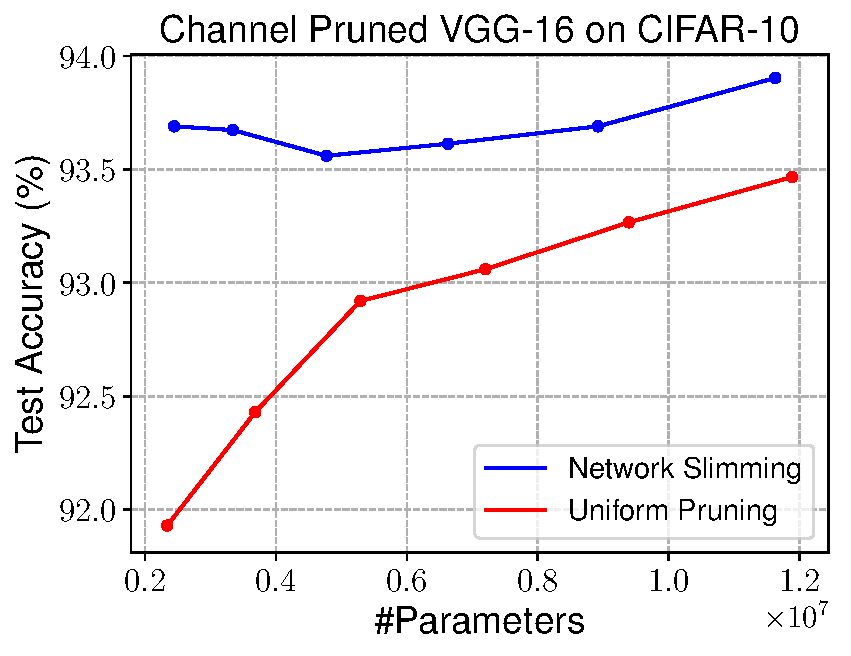
\includegraphics[width=\textwidth]{figures/cifar10-vgg16-slimming.pdf}
 \label{arch-search-a1}
 \end{subfigure}
\end{minipage}
\begin{minipage}{.47\textwidth}
 \begin{subfigure}{\textwidth}
 \centering
 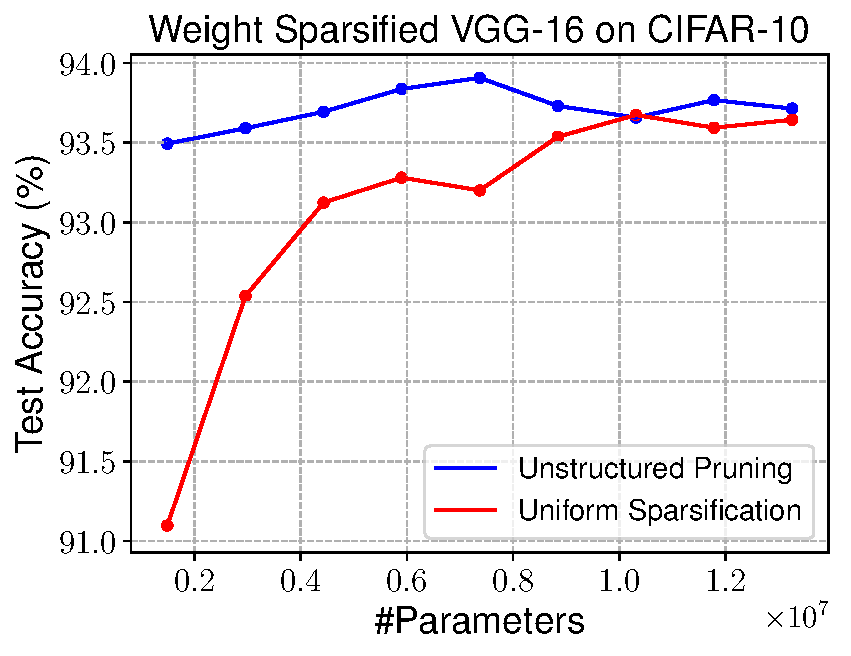
\includegraphics[width=\textwidth]{figures/cifar10-vgg16-weight-level-3.pdf}
 \label{arch-search-b1}
 \end{subfigure}
\end{minipage}
    \vspace{-3ex}
    \caption{
      Pruned architectures obtained by different approaches, all \emph{trained from scratch}, averaged over 5 runs.  
      Architectures obtained by  automatic pruning methods (\emph{Left:} Network Slimming \citep{liu2017learning}, \emph{Right:} Unstructured pruning \citep{han2015learning}) have better parameter efficiency than uniformly pruning channels or sparsifying weights in the whole network. }  
    \label{arch-search}
    \vspace{-1ex}
\end{figure*}



\setlength{\tabcolsep}{6pt}
\renewcommand{\arraystretch}{1.2}
\begin{table*}[!ht]%
% \begin{table*}[!ht]
% \resizebox{0.35\textwidth}{!}{
\begin{minipage}[b]{0.57\textwidth}%
% \begin{footnotesize}
\centering
% \vspace{1ex}
\resizebox{1.0\textwidth}{!}{
\begin{tabular}{c|cc||c|cc}
\hline
Layer & Width & Width*       & Layer & Width & Width*       \\ \hline
1     & 64    & 39.0$\pm$3.7  & 8     & 512   & 217.3$\pm$6.6 \\
2     & 64    & 64.0$\pm$0.0  & 9     & 512   & 120.0$\pm$4.4 \\
3     & 128   & 127.8$\pm$0.4 & 10    & 512   & 63.0$\pm$1.9  \\
4     & 128   & 128.0$\pm$0.0 & 11    & 512   & 47.8$\pm$2.9  \\
5     & 256   & 255.0$\pm$1.0 & 12    & 512   & 62.0$\pm$3.4  \\
6     & 256   & 250.5$\pm$0.5 & 13    & 512   & 88.8$\pm$3.1  \\
7     & 256   & 226.0$\pm$2.5 & Total & 4224  & 1689.2        \\ \hline
\end{tabular}
}
\vspace{1ex}
\captionof{table}{Network architectures obtained by pruning 60\% channels on VGG-16 (in total 13 conv-layers) using Network Slimming. Width and Width* are number of channels in the original and pruned architectures, averaged over 5 runs.}
\label{width}
\end{minipage}
\hspace{0.6ex}
\begin{minipage}[b]{0.40\textwidth}%
\centering
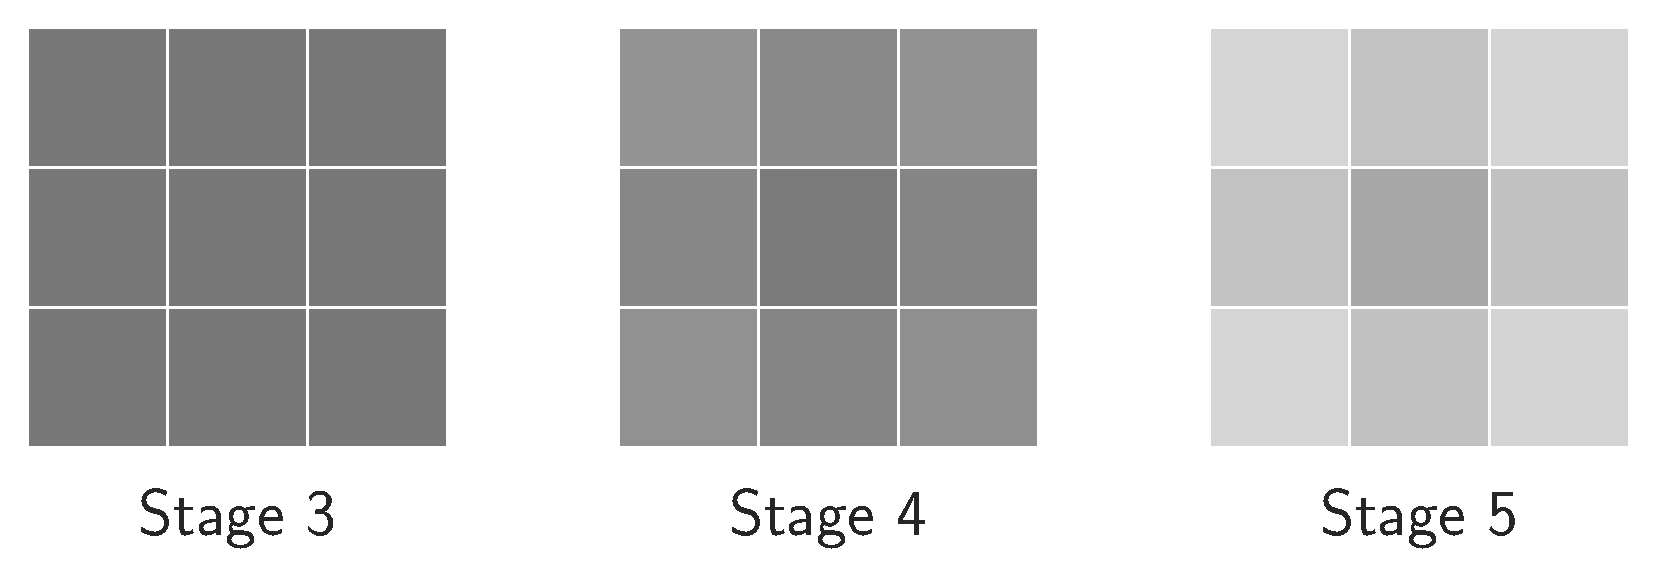
\includegraphics[width=1.\textwidth]{figures/heatmap.pdf}
\vspace{3.3ex}
\captionof{figure}{The average sparsity pattern of all 3$\times$3 convolutional kernels in certain layer stages in a unstructured pruned VGG-16. Darker color means higher probability of weight being kept.}
\vspace{-0.5ex}
\label{sparsity}
\end{minipage}
\vspace{-3ex}
\end{table*}
% \end{table*}

We also found the channel/weight pruned architectures exhibit very consistent patterns (see \autoref{width} and Figure \ref{sparsity}). 
This suggests the original large models may be redundantly designed for the task and the pruning algorithm can help us improve the efficiency. 
This also confirms the value of automatic pruning methods for searching efficient models on the architectures evaluated.


\begin{figure*}[!ht]
\centering
% \vspace{-2.5ex}
\begin{minipage}{.325\textwidth}
 \begin{subfigure}{\textwidth}
 \centering
 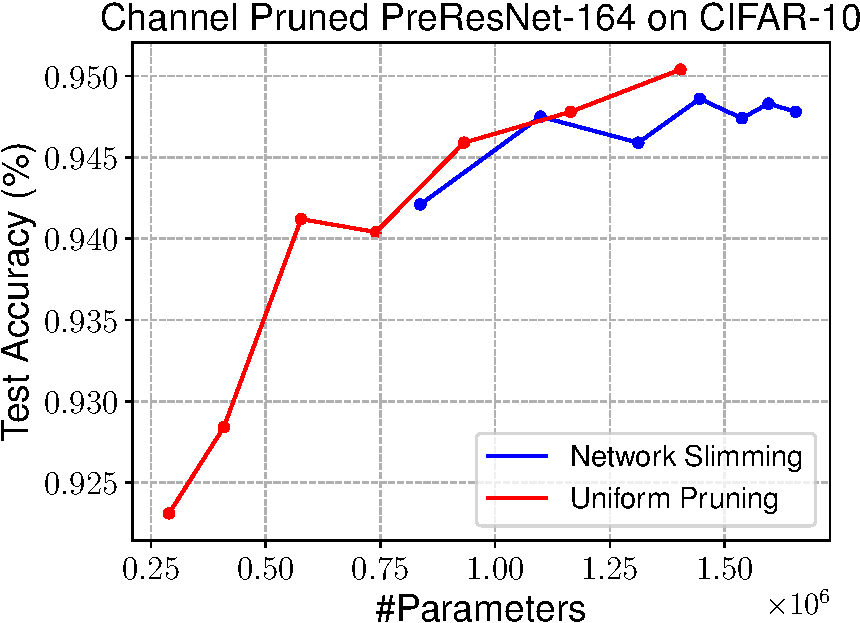
\includegraphics[width=\textwidth]{figures/slimming-preresnet-164-cifar10-crop.pdf}
%  \caption{}
%  \label{arch-search-a}
 \end{subfigure}
\end{minipage}
\begin{minipage}{.325\textwidth}
 \begin{subfigure}{\textwidth}
 \centering
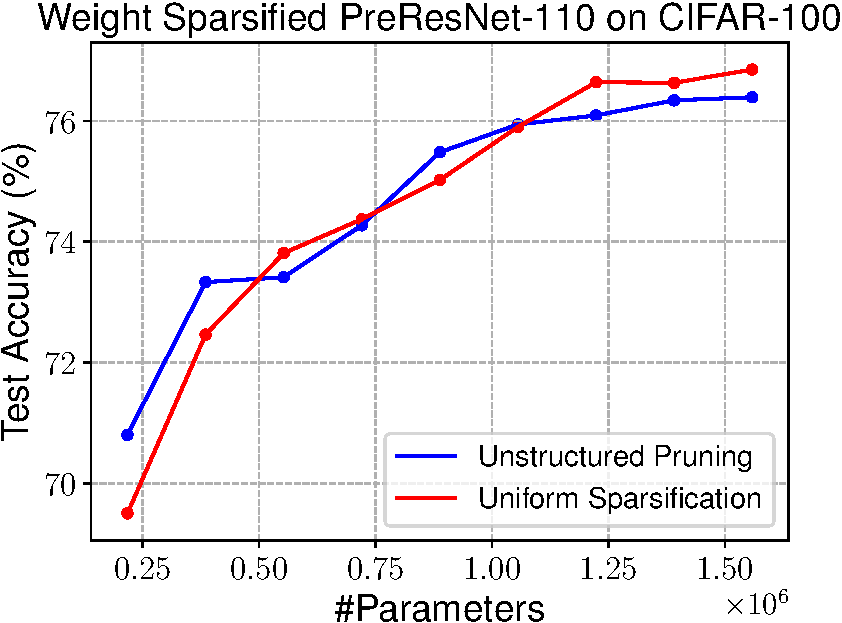
\includegraphics[width=\textwidth]{figures/weight-level-preresnet-110-cifar100-crop.pdf}
 \end{subfigure}
\end{minipage}
\begin{minipage}{.325\textwidth}
 \begin{subfigure}{\textwidth}
 \centering
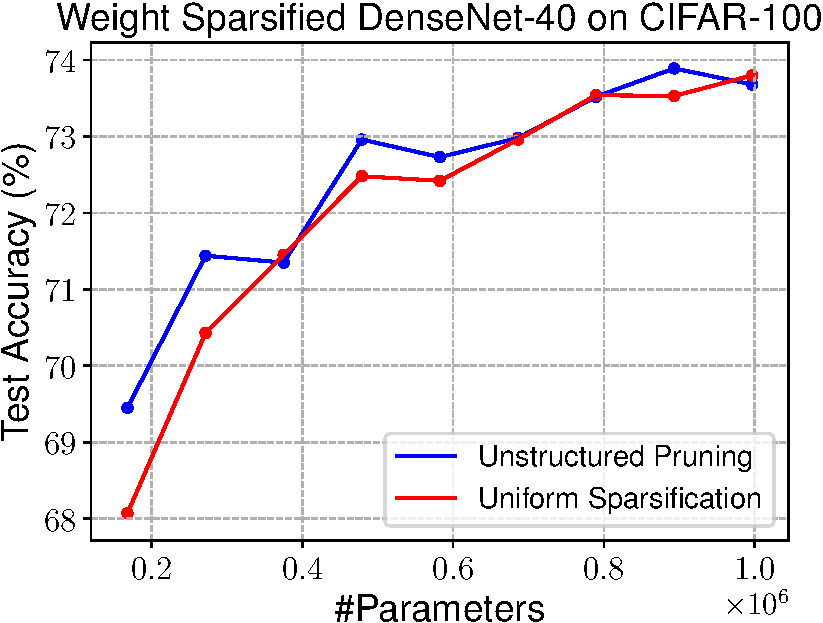
\includegraphics[width=\textwidth]{figures/weight-level-densenet-40-cifar100-crop.pdf}
 \end{subfigure}
\end{minipage}
    \vspace{-1ex}
    \caption{
      Pruned architectures obtained by different approaches, \emph{all trained from scratch}, averaged over 5 runs. \emph{Left:} Results for PreResNet-164 pruned on CIFAR-10 by Network Slimming~\citep{liu2017learning}. \emph{Middle} and \emph{Right}: Results for PreResNet-110 and DenseNet-40 pruned on CIFAR-100 by unstructured pruning~\citep{han2015learning}. 
    }
    \label{arch-search-negative}
% \vspace{-1.5ex}
\end{figure*}

\textbf{More Analysis.} However, there also exist cases where the architectures obtained by pruning are not better than uniformly pruned ones.
% and we defer the results and analysis in Appendix \ref{sec:additional} due to space limit. Continuing on \autoref{sec:arch}, 
We present such results in 
\autoref{arch-search-negative}, where the architectures obtained by pruning (blue) are not significantly more efficient than uniform pruned architectures (red). This phenomenon happens more likely on modern architectures like ResNets and DenseNets. When we investigate the sparsity patterns of those pruned architectures (shown in Table \ref{sparsity-5}, \ref{sparsity-6} and \ref{sparsity-8} in  Appendix~\ref{sec:additional}), we find that they exhibit near-uniform sparsity patterns across stages, which might be the reason why it can only perform on par with uniform pruning. In contrast, for VGG, the pruned sparsity patterns can always beat the uniform ones as shown in \autoref{arch-search} and \autoref{arch-search-2}. We also show the sparsity patterns of VGG pruned by Network Slimming~\citep{liu2017learning} in \autoref{sparsity-2} of Appendix~\ref{sec:additional}, and they are rather far from uniform. Compared to ResNet and DenseNet, we can see that VGG's redundancy is rather imbalanced across layer stages. Network pruning techniques may help us identify the redundancy better in the such cases.

\vspace{1.5ex}
\textbf{Generalizable Design Principles from Pruned Architectures.} Given that the automatically discovered architectures tend to be parameter efficient on the VGG networks, one may wonder: can we derive generalizable principles from them on how to design a better architecture? We conduct several experiments to answer this question.


\begin{figure*}[!ht]
\centering
% \vspace{-2.5ex}
\begin{minipage}{.47\textwidth}
 \begin{subfigure}{\textwidth}
 \centering
 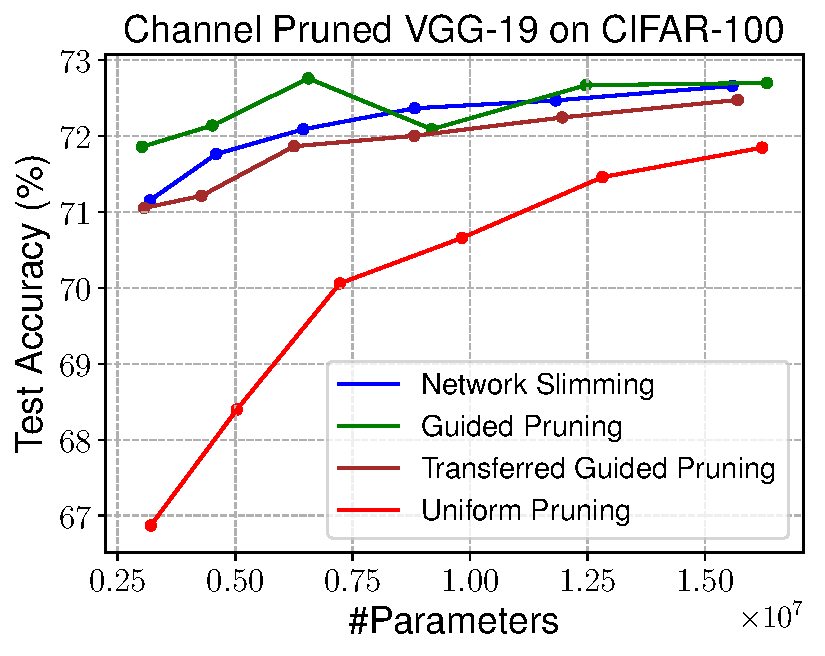
\includegraphics[width=\textwidth]{figures/cifar100-vgg19-slimming.pdf}
%  \caption{}
%  \label{arch-search-a}
 \end{subfigure}
\end{minipage}
\begin{minipage}{.47\textwidth}
 \begin{subfigure}{\textwidth}
 \centering
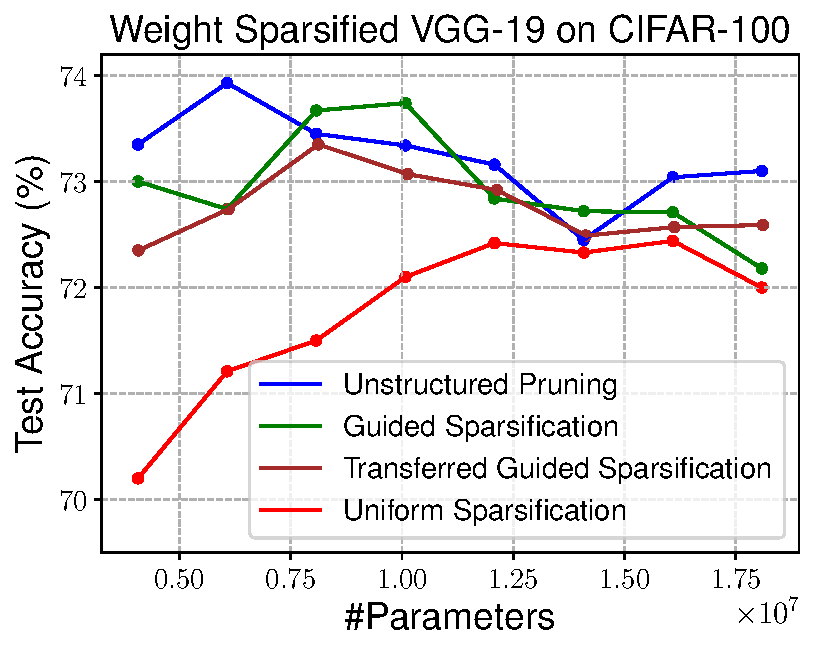
\includegraphics[width=\textwidth]{figures/cifar100-vgg19-transfer.pdf}
%  \caption{}
%  \label{arch-search-b}
 \end{subfigure}
\end{minipage}
    \vspace{-1ex}
    \caption{
      Pruned architectures obtained by different approaches, \emph{all trained from scratch}, averaged over 5 runs.
      ``Guided Pruning/Sparsification'' means using the average sparsity patterns in each layer stage  to design the network; ``Transferred Guided Pruning/Sparsification'' means using the sparsity patterns obtained by a pruned VGG-16 on CIFAR-10, to design the network for VGG-19 on CIFAR-100. 
    Following the design guidelines provided by the pruned architectures, we achieve better parameter efficiency, even when the guidelines are transferred from another dataset and model.}
    \label{arch-search-2}
\end{figure*}


For Network Slimming, we use the average number of channels in each layer stage (layers with the same feature map size) from pruned architectures to construct a new set of architectures, and we call this approach ``Guided Pruning'';
for magnitude-based pruning, we analyze the sparsity patterns (Figure \ref{sparsity}) in the pruned architectures,
and apply them to construct a new set of sparse models, which we call ``Guided Sparsification''. The results are shown in \autoref{arch-search-2}. It can be seen that for both Network Slimming (\autoref{arch-search-2} left) and unstructured pruning (\autoref{arch-search-2} right), guided design of architectures (green) can perform on par with pruned architectures (blue).

Interestingly, these guided design patterns can sometimes be transferred to a different VGG-variant and/or dataset. In \autoref{arch-search-2}, we distill the patterns of pruned architectures from VGG-16 on CIFAR-10 and apply them to design efficient VGG-19 on CIFAR-100. These sets of architectures are denoted as ``Transferred Guided Pruning/Sparsification''. We can observe that they (brown) may sometimes be slightly worse than architectures directly pruned (blue), but are significantly better than uniform pruning/sparsification (red). In these cases, one does not need to train a large model  to obtain an efficient model as well, as transferred design patterns can help us achieve the efficiency directly. 

\vspace{1.5ex}
\textbf{Discussions with Conventional Architecture Search Methods.}  Popular techniques for network architecture search include reinforcement learning \citep{rl1, rl2} and evolutionary algorithms \citep{genetic,liu2017hierarchical}. In each iteration, a randomly initialized network is trained and evaluated to guide the search, and the search process usually requires thousands of iterations to find the goal architecture. In contrast, using network pruning as architecture search  only requires a one-pass training, however the search space is restricted to the set of all ``sub-networks'' inside a large network, whereas traditional methods can search for more variations, e.g., activation functions or different layer orders.

Recently, \cite{gordon2018morphnet} uses a similar pruning technique to Network Slimming \citep{liu2017learning} to automate the design of network architectures; \cite{amc} prune channels using reinforcement learning and automatically compresses the architecture. On the other hand, in the network architecture search literature, sharing/inheriting trained parameters \citep{sharing,darts} during searching has become a popular approach for  reducing the training budgets, but once the target architecture is found, it is still trained from scratch to maximize the accuracy. 
